% GNUPLOT: LaTeX picture with Postscript
\begingroup
  \makeatletter
  \providecommand\color[2][]{%
    \GenericError{(gnuplot) \space\space\space\@spaces}{%
      Package color not loaded in conjunction with
      terminal option `colourtext'%
    }{See the gnuplot documentation for explanation.%
    }{Either use 'blacktext' in gnuplot or load the package
      color.sty in LaTeX.}%
    \renewcommand\color[2][]{}%
  }%
  \providecommand\includegraphics[2][]{%
    \GenericError{(gnuplot) \space\space\space\@spaces}{%
      Package graphicx or graphics not loaded%
    }{See the gnuplot documentation for explanation.%
    }{The gnuplot epslatex terminal needs graphicx.sty or graphics.sty.}%
    \renewcommand\includegraphics[2][]{}%
  }%
  \providecommand\rotatebox[2]{#2}%
  \@ifundefined{ifGPcolor}{%
    \newif\ifGPcolor
    \GPcolortrue
  }{}%
  \@ifundefined{ifGPblacktext}{%
    \newif\ifGPblacktext
    \GPblacktexttrue
  }{}%
  % define a \g@addto@macro without @ in the name:
  \let\gplgaddtomacro\g@addto@macro
  % define empty templates for all commands taking text:
  \gdef\gplbacktext{}%
  \gdef\gplfronttext{}%
  \makeatother
  \ifGPblacktext
    % no textcolor at all
    \def\colorrgb#1{}%
    \def\colorgray#1{}%
  \else
    % gray or color?
    \ifGPcolor
      \def\colorrgb#1{\color[rgb]{#1}}%
      \def\colorgray#1{\color[gray]{#1}}%
      \expandafter\def\csname LTw\endcsname{\color{white}}%
      \expandafter\def\csname LTb\endcsname{\color{black}}%
      \expandafter\def\csname LTa\endcsname{\color{black}}%
      \expandafter\def\csname LT0\endcsname{\color[rgb]{1,0,0}}%
      \expandafter\def\csname LT1\endcsname{\color[rgb]{0,1,0}}%
      \expandafter\def\csname LT2\endcsname{\color[rgb]{0,0,1}}%
      \expandafter\def\csname LT3\endcsname{\color[rgb]{1,0,1}}%
      \expandafter\def\csname LT4\endcsname{\color[rgb]{0,1,1}}%
      \expandafter\def\csname LT5\endcsname{\color[rgb]{1,1,0}}%
      \expandafter\def\csname LT6\endcsname{\color[rgb]{0,0,0}}%
      \expandafter\def\csname LT7\endcsname{\color[rgb]{1,0.3,0}}%
      \expandafter\def\csname LT8\endcsname{\color[rgb]{0.5,0.5,0.5}}%
    \else
      % gray
      \def\colorrgb#1{\color{black}}%
      \def\colorgray#1{\color[gray]{#1}}%
      \expandafter\def\csname LTw\endcsname{\color{white}}%
      \expandafter\def\csname LTb\endcsname{\color{black}}%
      \expandafter\def\csname LTa\endcsname{\color{black}}%
      \expandafter\def\csname LT0\endcsname{\color{black}}%
      \expandafter\def\csname LT1\endcsname{\color{black}}%
      \expandafter\def\csname LT2\endcsname{\color{black}}%
      \expandafter\def\csname LT3\endcsname{\color{black}}%
      \expandafter\def\csname LT4\endcsname{\color{black}}%
      \expandafter\def\csname LT5\endcsname{\color{black}}%
      \expandafter\def\csname LT6\endcsname{\color{black}}%
      \expandafter\def\csname LT7\endcsname{\color{black}}%
      \expandafter\def\csname LT8\endcsname{\color{black}}%
    \fi
  \fi
  \setlength{\unitlength}{0.0500bp}%
  \begin{picture}(7200.00,5040.00)%
    \gplgaddtomacro\gplbacktext{%
      \csname LTb\endcsname%
      \put(1056,2520){\makebox(0,0)[r]{\strut{}$0.4$}}%
      \put(1056,3165){\makebox(0,0)[r]{\strut{}$0.5$}}%
      \put(1056,3809){\makebox(0,0)[r]{\strut{}$0.6$}}%
      \put(1056,4454){\makebox(0,0)[r]{\strut{}$0.7$}}%
      \put(1369,2300){\makebox(0,0){\strut{}}}%
      \put(1791,2300){\makebox(0,0){\strut{}}}%
      \put(2394,2300){\makebox(0,0){\strut{}}}%
      \put(2997,2300){\makebox(0,0){\strut{}}}%
      \put(418,3648){\rotatebox{-270}{\makebox(0,0){\strut{}$<\tilde{\phi}_{local}>$}}}%
      \put(3819,3648){\rotatebox{-270}{\makebox(0,0){\strut{}}}}%
      \put(2394,4666){\makebox(0,0){\strut{}}}%
      \put(2394,4665){\makebox(0,0){\strut{}}}%
      \put(264,2190){\makebox(0,0)[l]{\strut{}}}%
    }%
    \gplgaddtomacro\gplfronttext{%
      \put(2557,4537){\makebox(0,0){\strut{}Experiments}}%
    }%
    \gplgaddtomacro\gplbacktext{%
      \csname LTb\endcsname%
      \put(3468,2520){\makebox(0,0)[r]{\strut{}}}%
      \put(3468,3165){\makebox(0,0)[r]{\strut{}}}%
      \put(3468,3809){\makebox(0,0)[r]{\strut{}}}%
      \put(3468,4454){\makebox(0,0)[r]{\strut{}}}%
      \put(3781,2300){\makebox(0,0){\strut{}}}%
      \put(4203,2300){\makebox(0,0){\strut{}}}%
      \put(4806,2300){\makebox(0,0){\strut{}}}%
      \put(5409,2300){\makebox(0,0){\strut{}}}%
      \put(6231,3648){\rotatebox{-270}{\makebox(0,0){\strut{}$<\tilde{\phi}_{ngb}>$}}}%
      \put(4806,4666){\makebox(0,0){\strut{}}}%
      \put(4806,4665){\makebox(0,0){\strut{}}}%
      \put(3336,2190){\makebox(0,0)[l]{\strut{}}}%
    }%
    \gplgaddtomacro\gplfronttext{%
      \csname LTb\endcsname%
      \put(4669,3877){\makebox(0,0)[r]{\strut{}$\phi=0.497$}}%
      \csname LTb\endcsname%
      \put(4669,4097){\makebox(0,0)[r]{\strut{}$\phi=0.535$}}%
      \csname LTb\endcsname%
      \put(4669,4317){\makebox(0,0)[r]{\strut{}$\phi=0.555$}}%
      \csname LTb\endcsname%
      \put(4669,4537){\makebox(0,0)[r]{\strut{}$\phi=0.576$}}%
    }%
    \gplgaddtomacro\gplbacktext{%
      \csname LTb\endcsname%
      \put(1056,704){\makebox(0,0)[r]{\strut{}$0.4$}}%
      \put(1056,1223){\makebox(0,0)[r]{\strut{}$0.5$}}%
      \put(1056,1741){\makebox(0,0)[r]{\strut{}$0.6$}}%
      \put(1056,2260){\makebox(0,0)[r]{\strut{}$0.7$}}%
      \put(1369,484){\makebox(0,0){\strut{}$-0.17$}}%
      \put(1791,484){\makebox(0,0){\strut{}$-0.1$}}%
      \put(2394,484){\makebox(0,0){\strut{}$0$}}%
      \put(2997,484){\makebox(0,0){\strut{}$0.1$}}%
      \put(418,1611){\rotatebox{90}{\makebox(0,0){\strut{}$<\phi_{local}>$}}}%
      \put(2394,154){\makebox(0,0){\strut{}$w_6$}}%
      \put(2394,2409){\makebox(0,0){\strut{}}}%
      \put(2394,2408){\makebox(0,0){\strut{}}}%
      \put(264,110){\makebox(0,0)[l]{\strut{}}}%
    }%
    \gplgaddtomacro\gplfronttext{%
      \put(2161,2305){\makebox(0,0){\strut{}Simulations}}%
      \csname LTb\endcsname%
      \put(2740,1865){\makebox(0,0)[r]{\strut{}$\phi=0.548$ }}%
      \csname LTb\endcsname%
      \put(2740,2085){\makebox(0,0)[r]{\strut{}$\phi=0.568$ }}%
    }%
    \gplgaddtomacro\gplbacktext{%
      \csname LTb\endcsname%
      \put(3468,704){\makebox(0,0)[r]{\strut{}}}%
      \put(3468,1223){\makebox(0,0)[r]{\strut{}}}%
      \put(3468,1741){\makebox(0,0)[r]{\strut{}}}%
      \put(3468,2260){\makebox(0,0)[r]{\strut{}}}%
      \put(3781,484){\makebox(0,0){\strut{}$-0.17$}}%
      \put(4203,484){\makebox(0,0){\strut{}$-0.1$}}%
      \put(4806,484){\makebox(0,0){\strut{}$0$}}%
      \put(5409,484){\makebox(0,0){\strut{}$0.1$}}%
      \put(6231,1611){\rotatebox{90}{\makebox(0,0){\strut{}$<\phi_{ngb}>$}}}%
      \put(4806,154){\makebox(0,0){\strut{}$w_6$}}%
      \put(4806,2409){\makebox(0,0){\strut{}}}%
      \put(4806,2408){\makebox(0,0){\strut{}}}%
      \put(3336,110){\makebox(0,0)[l]{\strut{}}}%
    }%
    \gplgaddtomacro\gplfronttext{%
      \csname LTb\endcsname%
      \put(4669,1865){\makebox(0,0)[r]{\strut{}$\phi=0.487$ }}%
      \csname LTb\endcsname%
      \put(4669,2085){\makebox(0,0)[r]{\strut{}$\phi=0.507$ }}%
      \csname LTb\endcsname%
      \put(4669,2305){\makebox(0,0)[r]{\strut{}$\phi=0.528$ }}%
    }%
    \gplbacktext
    \put(0,0){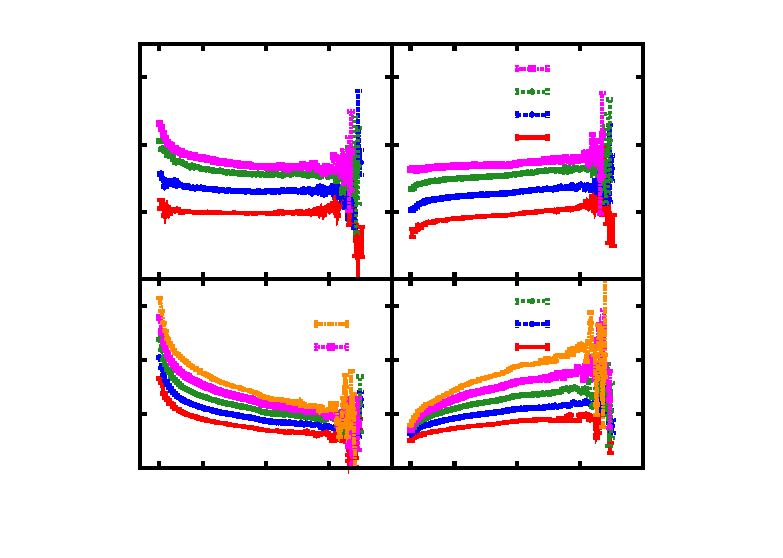
\includegraphics{phi_w6_xpsim_total}}%
    \gplfronttext
  \end{picture}%
\endgroup
